\documentclass[dvipdfmx]{jsarticle}
\usepackage{amsmath,amssymb}
\usepackage[dvipdfmx]{graphicx}
\usepackage{siunitx}
\usepackage{float}
\usepackage{tikz}
\usepackage{circuitikz}
\usepackage{threeparttable}
\usepackage{tabularx}
\usepackage{amsmath}
\usepackage{amssymb}
\graphicspath{{./figure/}}
\newcolumntype{Y}{&gt;{\centering\arraybackslash}X} %中央揃え

\begin{document}
\section{目的}

我々が日常的に電力として利用している電気の多くは交流である。
また回路理論を学ぶ上で、交流及び交流回路の基本的な性質の理解は必要不可欠である。
本実験では、以下の3点を理解することを目的とする。

\begin{itemize}
\item
  交流電圧と周波数の測定方法
\item
  交流電圧波形の解析による交流の諸性質
\item
  交流回路における受動素子の構造と働き
\end{itemize}

\section{原理}

\subsection{正弦波交流の表式}

正弦波交流電圧\(v\)や電流\(i\)は次のような数式で表される。

\begin{eqnarray}
v = V_m\sin(\omega t + \theta_v)\\
i = I_m\sin(\omega t + \theta_i)
\end{eqnarray}

ここでは、\(V_m\)は電圧の最大値、\(\theta_v\)は電圧の位相角、\(\theta_i\)は電流の
位相角、\(t\)は時間\(\omega\)は角周波数を表す。
また、角周波数\(\omega\)と周期\(T\)、周波数\(f\)の関係は次のような式で表される。

\begin{equation}
\omega = \frac{2}{\pi} = 2\pi f[\rm rad/s]
\end{equation}

\subsubsection{瞬時値と実効値}

ある時刻の交流の大きさを瞬時値と言う。実効値は、瞬時値の2乗を1周期の間平均した
値の平方根として定義され、交流の大きさを表すときに使われる。
実効値の物理的な意味は、「交流電圧(電流)を抵抗に加えたときに消費する電力が、
その実効値と同じ大きさの直流電圧(電流)を加えたときの消費電力と等しくなる。」
ということである。 実効値は次の式で求められる。

\begin{eqnarray}
V = \frac{V_m}{\sqrt{2}}, I = \frac{I_m}{\sqrt2}
\end{eqnarray}

\subsection{各種計測器で測定可能な電気的諸量}

本実験で使用する計測器で測定できる電気量を表\ref{tb:table_dennki}に示す。

\begin{table}[h]
  \caption{各種計測器で測定可能な電気的諸量}
  \label{tb:table_dennki}
  \begin{threeparttable}
    \begin{tabular}{|c|c|c|c|c|c|}\hline 
      \multicolumn{2}{|c|}{電気量} & アナログ回路計 & ディジタルマルチメータ & 交流電子電圧計 & オシロスコープ \\ \hline
      \multicolumn{2}{|c|}{抵抗} & ○\footnotemark[2] & ◎\footnotemark[1] & ×\footnotemark[4] & × \\ \cline{1-6}
      直流 & 電圧 & ○ & ◎ & × & △\footnotemark[3]\\ \cline{2-6}
       & 電流 & ○ & ◎ & × & ×\\ \hline
      交流 & 電圧 & ○ & ○ & ◎ & △\\ \cline{2-6}
       & 電流 & ○ & ○ & × & ×\\ \hline
      \multicolumn{2}{|c|}{周波数} & × & ◎ & × & △\\ \hline
      \multicolumn{2}{|c|}{波形} & ×  & ×  & ×  & ◎ \\ \hline 
    \end{tabular}
    \begin{tablenotes}\footnotesize
      \item[1] 優
      \item[2] 良
      \item[3] 可
      \item[4] 不可
      \end{tablenotes}
\end{threeparttable}
\end{table}
\subsection{リサジュー図形を用いた位相差の測定}

リサジュー図形とは互いに直行する単振動が平面上に描く軌跡である。互いに直行する単振動を

\begin{eqnarray}
  x(t) = A_1\sin(\omega_1 t + \theta_1) \\
	y(t) = A_2\sin(\omega_2 t + \theta_2) 
\end{eqnarray}

とする時、点$(x(t), y(t))を様々なtの値に対して、X-Y平面上$
でプロットして得られる図形がリサジュー図形である。

$x(t)とy(t)$の周波数が等しい場合、リサジュー図形を用いて位相差を求めることができる。

\begin{eqnarray}
  |\sin(\theta_1 - \theta_2)| = \sin^{-1} \frac{b}{a}
\end{eqnarray}

$a$は$x軸方向$の最大値と最小値の差、$b$は$y(t) = 0$を満たす2点の距離である。

\subsection{円筒形コイルのインダクタンスと測定方法}
絶縁された電線を円筒形に一重に巻くことによって作られたコイルのインダクタンス$L$は
次式で与えられる。

\begin{eqnarray}
  L = K \frac{\pi^2 D^2 N^2}{l} \times 10^{-7}
\end{eqnarray}

$Dは直径、lは長さ、Nは巻き数、Kは長岡係数である。$長岡係数とは、直径と長さの比$D/l$で決まる
定数である。

\begin{figure}[h]
  \centering
  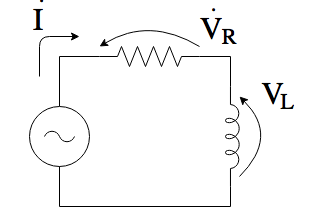
\includegraphics[scale=0.4]{RL_Series_Circut.png}
  \caption{RL直列回路}
  \label{fig:RL_Series_Circuit}
\end{figure}

図\ref{fig:RL_Series_Circuit}に示す
RL直列回路において電圧$\dot V_R, \dot V_L$の実効値(または最大値)と角周波数$\omega、抵抗R$
からインダクタンス$L$を以下の式から求める事ができる。

\begin{eqnarray}
  L = \frac{R}{\omega}\frac{|\dot V_R|}{|\dot V_L|}
\end{eqnarray}

\subsection{平行平板コンデンサのキャパシタンスと測定方法}
同じ形の2枚の金属板を平行に配置する事によって作られた平行平板コンデンサのキャパシタンス
$C$は次式で与えられる。

\begin{eqnarray}
  C = \epsilon_0 \epsilon_r \frac{S}{d}
\end{eqnarray}

$\epsilon_0は真空中の誘電率、\epsilon_rは金属板間を満たす物質の比誘電率、Sは金属板の
面積、dは金属板間の距離である。$

\begin{figure}[h]
  \centering
  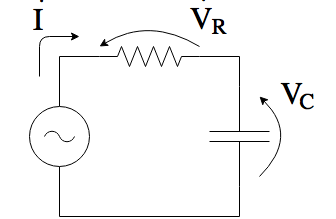
\includegraphics[scale=0.4]{RC_Series_Circuit.png}
  \caption{RC直列回路}
  \label{fig:RC_Series_Circuit}
\end{figure}

図\ref{fig:RC_Series_Circuit}に示すRC直列回路において、電圧$\dot V_R, \dot V_C$の実効値(または最大値)と角周波数$\omega、抵抗R$
から、キャパシタンス$C$を以下の式から求めることができる。

\begin{eqnarray}
  C = \frac{1}{\omega R} \frac{|\dot V_R|}{|\dot V_C|}
\end{eqnarray}

\section{実験方法}
\subsection{各種計測器による交流電圧の測定}
以下の手順に従って、図\ref{fig:experimental_circuit}に示す回路において各種計測器を用いて交流電圧を測定した。
\begin{itemize}
  \item [(1)]ブレッドボードを用いて、図の回路を作製せよ。
  \item [(2)]オシロスコープで図中の電圧$v$を測定し、オシロスコープに表示される
            電圧の最大値が3 [V]、周波数が1 [kHz]になるように発振器の出力を調節する。
  \item [(3)]電圧$v$が測定できるように、交流電子電圧計を回路につなぎ、計測値が2[V]に
              なるよう発振器の電圧ツマミを調節する。
  \item [(4)](3)の状態での各種計測器による電圧測定値を表に記録する。
  \item [(5)]発振器の周波数を調整してオシロスコープの周波数表示が表\ref{tb:result2}に示す値になるようにし、
            各周波数における電圧を表に示す計測器で測定する。この実験では、発振器の電圧調整ツマミは
            (4)の状態から変化させない。
\end{itemize}
\begin{figure}[h]
  \centering
  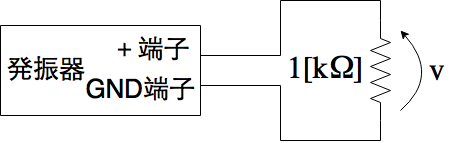
\includegraphics[scale=0.4]{experimental_circuit.png}
  \caption{実験回路}
  \label{fig:experimental_circuit}
\end{figure}

\subsection{オシロスコープを用いた交流電圧の取得}
\subsubsection{測定データの取得}
前の実験「各種計測器による交流電圧の測定」(3)の状態にする。オシロスコープを
用いて測定データを保存する。また、表に実験に使用した抵抗の抵抗値と周波数を示す。
\subsubsection{測定データの利用}
\begin{itemize}
  \item [(1)]表計算ソフトウェアを用いて保存された.cvsファイルを開き、.xlsxファイルとして保存する。
  \item [(2)]表計算ソフトウェアの機能を用いて、オシロスコープで測定されたデータから、電圧波形のグラフを作成する。
            グラフは、横軸を時間、縦軸を電圧とする。
\end{itemize}
\subsection{表計算ソフトウェアを用いた交流の解析}
第3.2節で取得したデータを用いて、表計算ソフトウェア上で以下の解析を行う。
\begin{itemize}
  \item [(1)]データ保存時に交流電子電圧計で測定した測定値(実効値)を記録する。
        またその電圧値から、計算によって電圧の最大値と半周期分の平均値、及び
        電流の実効値を求め、記録する。
  \item [(2)]測定データから周期、周波数を求める。
  \item [(3)]半周気分の瞬時値から、最大値と平均値を求め、記録する。
  \item [(4)]半周期文の瞬時電圧値の一つ一つの値を表で記録した抵抗値で除算する事により、半周期分の瞬時電流値を求める。
  \item [(5)]電圧と電流の瞬時値から、半周期に渡っての電力の瞬時値を求める。
  \item [(6)]前項の瞬時電圧の半周期分の平均値を求め、記録する。また、求めた電力の平均値
            が、実行電圧値と実行電流値の積と等しくなることを確認する。
\end{itemize}

\subsection{瞬時電圧を表す式の導出と比較}
以下の手順に従って、測定データから瞬時電圧を表す式を求め、式から計算される
電圧値と測定値を比較する。
\begin{itemize}
  \item [(1)]第4.2節でオシロスコープで保存したデータから求めた周波数から、角周波数$\omega$を求める。
  \item [(2)]瞬時電圧の式$v(t) = V_m \sin(\omega t + \theta)$に前項の$\omega$を代入し、
              測定された交流電圧の瞬時値を表す式を求める。ただし$\theta = 0$とする。
  \item[(3)]列挙した時刻における位相$\omega t$を以下の式から求める事ができる。
  \item[(4)]各時刻における瞬時電圧値を、(2)で求めた式を用いて算出する。また、計算値と測定値を比較する。
\end{itemize}

\subsection{位相差の測定}
\begin{itemize}
  \item [(1)]図\ref{fig:experimental_circuit2}に示す回路を作製する
  \item [(2)]図中の電圧$V, V_1, V_2$をオシロスコープで測定し、データを保存する。
  \item [(3)](2)で保存したデータから、各電圧の最大と周波数を求める。
  \item [(4)]$VとV_1、VとV_2、V_1とV_2の組み合わせについて$、以下の二通りの方法で位相差を測定する。
    \begin{description}
      \item [正弦波の時間差から求める]正弦波が同じ位相になる点の時間差$\delta t$から位相差$\phi = \omega \delta t$を求める事ができる。
      \item [リサジュー図形から求める]リサジュー図形を用いて、2.3の原理に基づき位相差を求める。
    \end{description}
  \item[(5)]求めた各値から、各電圧の瞬時値を与える式を求める。ただし、位相角$\theta$はゼロとし、$V$を基準とし$V_1, V_2$の位相角を決定する。
\end{itemize}
\begin{figure}[h]
  \centering
  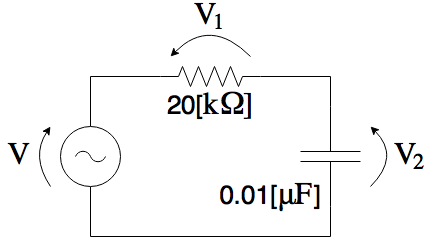
\includegraphics[scale=0.4]{experimental_circuit2.png}
  \caption{RC直列回路}
  \label{fig:experimental_circuit2}
\end{figure}

\subsection{インダクタンスの作成と測定}
\subsubsection{コイルの作製}
直径7.5 [cm]の塩化ビニル製のパイプとフォルマル線を用いて、25巻と50巻の二種類のコイルを作製する。
\subsubsection{インダクタンスの測定}
作製したコイルの内、25巻のものを$L_1$、50巻のものを$L_2$とする。
以下の四つの場合において、図\ref{fig:RL_Series_Circuit}のRL直列回路をブレッドボード上に作製し、
$|\dot V_R|, |\dot V_L|$を測定する。ただし、周波数は100 [kHz]、抵抗Rは$100 [\Omega]$とする。
\begin{itemize}
  \item [(1)]$L_1$のみ
  \item [(2)]$L_2$のみ
  \item [(3)]$L_1, L_2$の直列接続
  \item [(4)]$L_1, L_2$の並列接続
\end{itemize}
\subsection{キャパシタンスの制作と測定}
\subsubsection{コンデンサの作製}
アルミホイル、OHPシート、両面テープを用いて、極板の形状が5 [cm] $\times$ 5 [cm]と
10 [cm] $\times$ 5 [cm]の二種類のコンデンサを作製する。
\subsubsection{キャパシタンスの測定}
作製したコンデンサの内、極板形状が5 [cm] $\times$ 5 [cm]のものを$C_1$、
10 [cm] $\times$ 5 [cm]のものを$C_2$とする。
以下の四つの場合において、図\ref{fig:RC_Series_Circuit}のRC直列回路をブレッドボード上に作製し、
$|\dot V_R|, |\dot V_C|$を測定する。ただし、周波数は1 [kHz]、抵抗Rは500 $[k\Omega]$とする。
\begin{itemize}
  \item [(1)]$C_1$のみ
  \item [(2)]$C_2$のみ
  \item [(3)]$C_1, C_2$の直列接続
  \item [(4)]$C_1, C_2$の並列接続
\end{itemize}

\section{実験結果}
\subsection{各種計測器による交流電圧の測定}
交流電子電圧計が2Vの値を示すように調節した際の、実験の結果を表\ref{tb:result1}に示す。

\begin{table}[h]
   \caption{測定結果(1)}
   \label{tb:result1}
   \begin{tabularx}{\linewidth}{|X|X|X|X|X|}\hline
     オシロスコープ(最大値) & ディジタルマルチメータ(交流モード) & ディジタルマルチメータ(直流モード) & 交流電子電圧計 & アナログ回路計\\ \hline
     5.88 [V] & 2.043 [V] & 0.047[V] & 2.0[V] & 2.03[V]\\ \hline
  \end{tabularx}
\end{table}

また、周波数を変化させた際の結果を表に、そのグラフを図\ref{fig:result_graph}に示す。

\begin{table}
  \caption{測定結果(2)}
  \label{tb:result2}
  \begin{tabularx}{\linewidth}{|X|X|X|X|X|X|X|}\hline
      \multicolumn{3}{X}{周波数[Hz]} & \multicolumn{4}{X}{電圧[V]}\\ \hline
      設定値 & オシロスコープ & ディジタルマルチメータ(交流モード) & 交流電子電圧計 & オシロスコープ(最大値) & ディジタルマルチメータ(交流モード) & アナログ回路計(交流モード)\\ \hline
      100 & 100.4 & 100.2 & 1.93 & 5.88 & 2.03 & 2.02 \\ \hline
      200 & 200.8 & 201 & 1.96 & 5.88 & 2.02 & 2.01 \\ \hline
      500 & 497 & 497.2 & 1.98 & 5.88 & 2.012 & 2.01 \\ \hline
      1000 & 1002 & 1000 & 2.0 & 5.88 & 2.028 & 2.01 \\ \hline
      2000 & 2004 & 2004 & 1.96 & 5.88 & 2.009 & 2.01 \\ \hline
      5000 & 5000 & 4997 & 1.94 & 5.88 & 1.96 & 2.01 \\ \hline
      10000 & 10120 & 10120 & 1.94 & 5.88 & 1.837 & 2.01 \\ \hline
      20000 & 20040 & 20040 & 1.94 & 5.88 & 1.478 & 2.01 \\ \hline
      50000 & 50050 & 50040 & 1.94 & 5.88 & 0.678 & 2.0 \\ \hline
      100000 & 102000 & 測定不能 & 1.94 & 5.88 & 測定不能 & 1.99 \\ \hline
      200000 & 202000 & 測定不能 & 1.92 & 5.88 & 測定不能 & 1.94 \\ \hline
      500000 & 503000 & 測定不能 & 1.89 & 5.88 & 測定不能 & 1.81 \\ \hline
  \end{tabularx}
\end{table}

\begin{figure}[h]
  \centering
  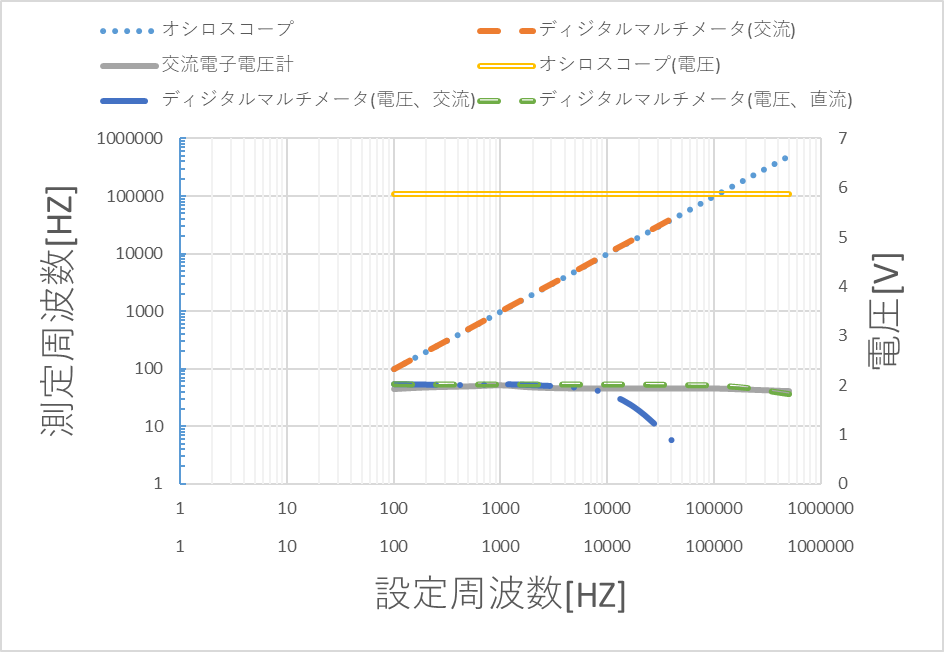
\includegraphics[scale=1]{image001.png}
  \caption{測定結果のグラフ}
  \label{fig:result_graph}
\end{figure}

\subsection{オシロスコープを用いた交流電圧の取得}
表計算ソフトウェアを用いて、測定データから作成したグラフを図\ref{fig:result_graph2}に示す。
\begin{figure}[h]
  \centering
  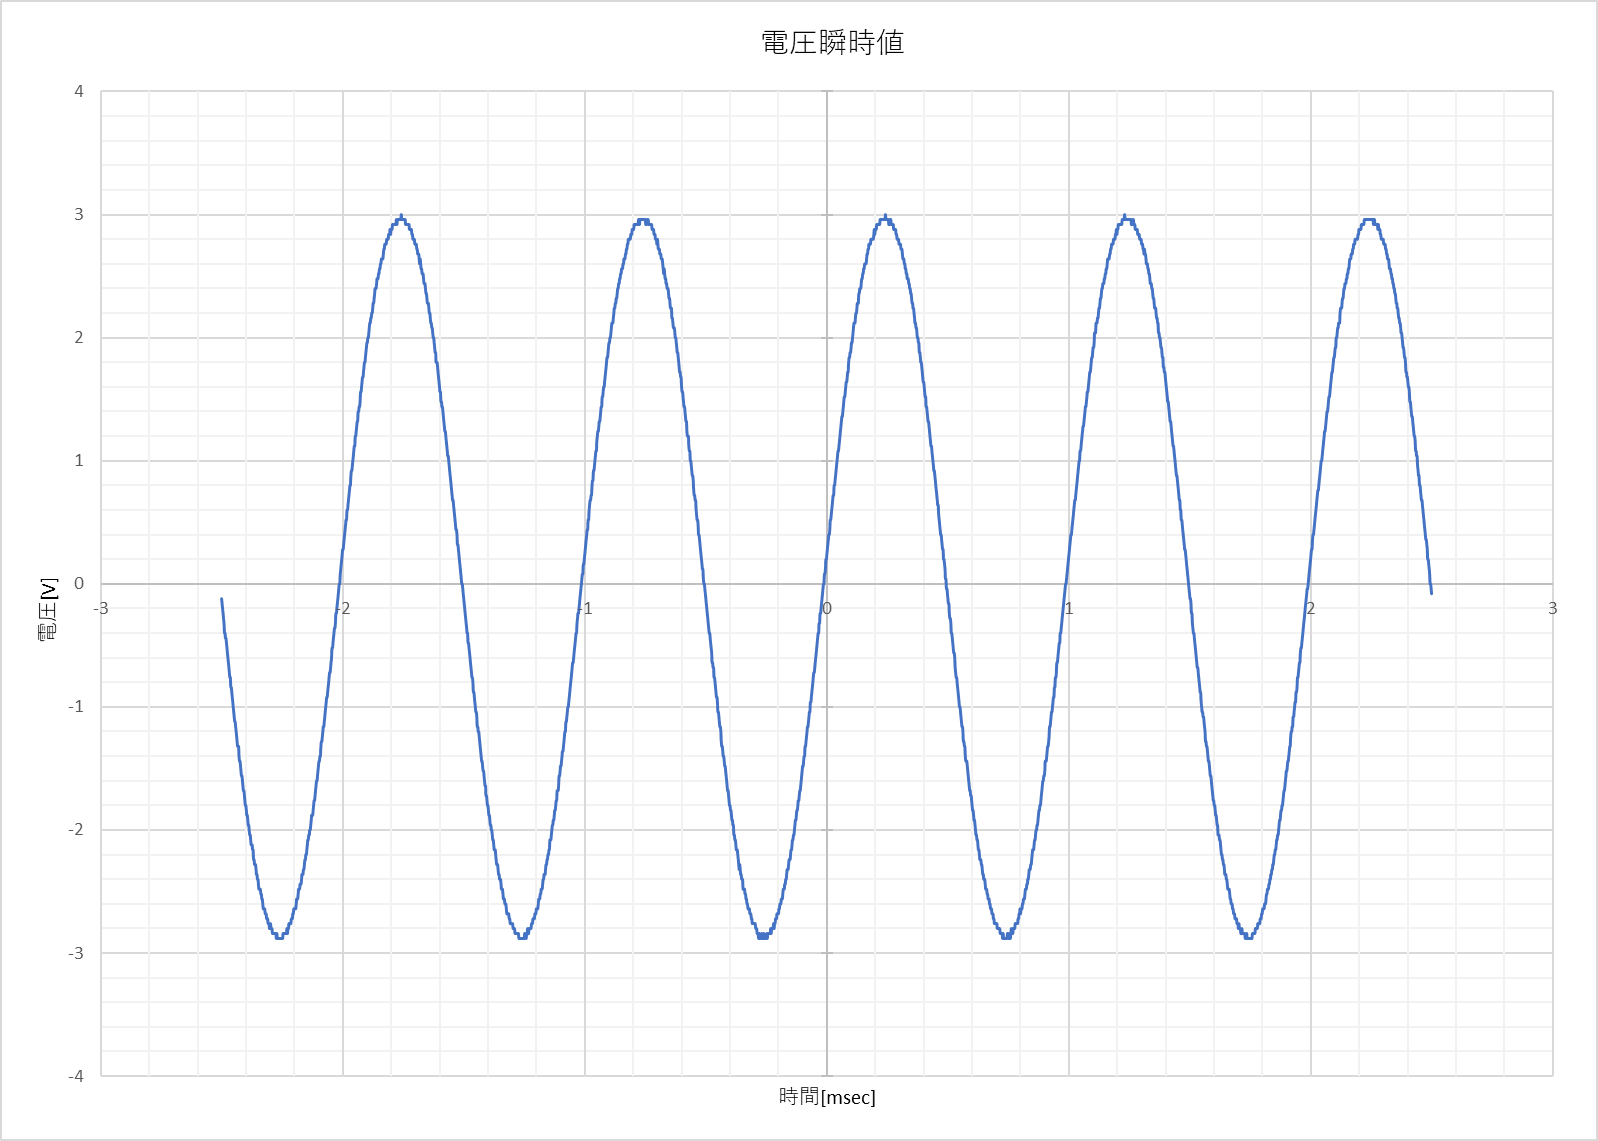
\includegraphics[scale=0.5]{image2.png}
  \caption{測定値から作成したグラフ}
  \label{fig:result_graph2}
\end{figure}

\section{表計算ソフトウェアを用いた交流の解析}
それぞれの測定値、計算値を表\ref{tb:result3}と表\ref{tb:result4}に示す。
\begin{table}[h]
  \caption{測定値及び計算値}
  \label{tb:result3}
  \begin{tabularx}{\linewidth}{|X|X|X|X|X|}\hline
    電圧実効値(交流電子電圧計で測定) & 周波数(オシロスコープで測定) & 電圧最大値(計算) & 半周期分の電圧平均値(計算) & 電流実効値(計算)\\ \hline
    2.0 [V] & 999 [Hz] & 2.83 [V] & 1.8006 [V] & 0.002014[A]\\ \hline 
  \end{tabularx}
\end{table}

\begin{table}[h]
  \caption{測定データから求めた値}
  \label{tb:result4}
  \begin{tabularx}{\linewidth}{|X|X|X|X|}\hline
    周波数 & 電圧最大値 & 半周期分の電圧平均値 & 半周期分の電力平均値\\ \hline
    1000 [Hz] & 3.0[V] & 1.89 [V] & 0.00472 [W]\\ \hline
 \end{tabularx}
\end{table}

\subsection{瞬時電圧の表す式の導出と比較}
導出した式は以下のようになった。
\begin{eqnarray}
  v(t) = 3\sin(6283.185t)
\end{eqnarray}
導出した式と測定値の比較を表\ref{tb:result5}に示す。
\begin{table}[h]
  \centering
  \caption{瞬時電圧の比較}
  \label{tb:result5}
  \begin{tabular}{|c|c|c|c|c|c|c|}\hline
    \multicolumn{2}{c}{時刻 [ms]} & 0.0 & 0.2 & 0.4 & 0.6 & 0.8\\ \cline{1-7}
    位相$\omega t$ & [rad] & 0 & 1.26 & 2.51 & 3.77 & 5.027\\ \cline{2-7}
    & [度] & 0 & 72.0 & 144 & 216 & 288\\ \hline
    \multicolumn{2}{c}{瞬時電圧(計算値) [V]} & 0 & 2.85 & 1.76 & -1.76 & -2.85\\ \hline
    \multicolumn{2}{c}{測定値} & 0.24 & 2.88 & 1.64 & -0.12 & -2.68\\ \hline
  \end{tabular}
\end{table}

\subsection{位相差の測定}
測定したデータを表\ref{tb:result6}に、位相差を表に示す。
\begin{table}
  \centering
  \caption{測定結果(3)}
  \label{tb:result6}
  \begin{tabular}{|c|c|c|c|}\hline
    & V & $V_1$ & $V_2$ \\ \hline
    最大値 [V] & 10.6 & 8.2 & 6.4\\ \hline
    周波数 [Hz] & 1000 & 1000 & 1000\\ \hline 
  \end{tabular}
\end{table}

\begin{table}
  \centering
  \caption{位相差}
  \label{tb:result7}
  \begin{tabular}{|c|c|c|c|}\hline
    & $V-V_1$ & $V-V_2$ & $V_1-V_2$ \\ \hline
    時間差から & & &\\ \hline
    リサジュー図形から & 0.7075 [rad]/40.54 [度] & 0.927 [rad]/53.1 [度] & 1.57 [rad]/90 [度]\\ \hline
  \end{tabular}
\end{table}

また、求めた値から、各電圧の瞬時値を与える式を表\ref{tb:result8}に示す。

\begin{table}[h]
  \centering
  \caption{瞬時値の式}
  \label{tb:result8}
  \begin{tabular}{|c|c|}\hline
    $V$ & $v(t) = 10.6\sin(6283.185t + 0)$ \\ \hline
    $V_1$ & $v(t) = 8.2\sin(6283.185t + 0.7075)$ \\ \hline
    $V_2$ & $v(t) = 10.6\sin(6283.185t + 0.927)$ \\ \hline
  \end{tabular}
\end{table}

\subsection{インダクタンスの制作と測定}
測定した電圧及び、求めたインダクタンスを表\ref{tb:result9}に示す。

\begin{table}[h]
  \centering
  \caption{インダクタンスの測定}
  \label{tb:result9}
  \begin{tabular}{|c|c|c|c|}\hline
    & $|\dot V_R|$ [V] & $|\dot V_L| [V]$ & $L$\\ \hline
    $L_1$のみ & 1.0 & 0.49 & 7.77$\times 10^{-5}$\\ \hline
    $L_2$のみ & 0.97 & 1.59 & 2.60$\times 10^{-4}$\\ \hline
    $L_1, L_2$直列接続 & 0.89 & 2.09 & 3.72$\times 10^{-4}$\\ \hline
    $L_1, L_2$並列接続 & 1.0 & 0.39 & 6.18$\times 10^{-5}$\\ \hline
  \end{tabular}
\end{table}

\subsection{キャパシタンスの制作と測定}
測定した電圧及び、求めたキャパシタンスを表\ref{tb:result10}に示す。
\begin{table}[h]
  \centering
  \caption{インダクタンスの測定}
  \label{tb:result10}
  \begin{tabular}{|c|c|c|c|}\hline
    & $|\dot V_R|$ [V] & $|\dot V_C| [V]$ & $C$\\ \hline
    $C_1$のみ & 0.96 & 6.2 & 4.86$\times 10^{-13}$\\ \hline
    $C_2$のみ & 0.42 & 6.0 & 2.20$\times 10^{-13}$\\ \hline
    $C_1, C_2$直列接続 & 0.00089 & 6.26 & 4.46$\times 10^{-16}$\\ \hline
    $C_1, C_2$並列接続 & 0.6 & 5.9 & 3.19$\times 10^{-13}$\\ \hline
  \end{tabular}
\end{table}

\section{考察}
\subsection{使用する機器の選び方や特性について注意するべきことについて}
\begin{itemize}
  \item 正確な交流の電圧を測定したい場合は、交流電子電圧計を使用すべきである。
  \item 正確な周波数を測定したい場合は、オシロスコープを使用するべきである。
  \item ディジタルマルチメータを利用する際は、高い周波数の時には正確な値が測定できないことに注意するべきである。
\end{itemize}

\subsection{電圧最大値$V_m$時に実効値が$\frac{V_m}{\sqrt{2}}$になることを示す}
\begin{eqnarray}
  I & = & \sqrt{\frac{1}{T} \int_0^T i^2 dt} = \sqrt{\frac{1}{T} \int_0^T {I_m}^2\sin^2(\omega t + \theta) dt}\nonumber \\
 & = &\sqrt{\frac{{I_m}^2}{T} \int_0^T \frac{1}{2} \{1 - \cos2(\omega t + \theta)\} dt}\nonumber \\
 & = & \sqrt{\frac{{I_m}^2}{2T} \left[t - \frac{1}{2\omega}\sin2(\omega t + \theta)\right]_0^T}\nonumber \\
 & = & \sqrt{\frac{{I_m}^2}{2T} \{T - \frac{1}{2\omega}\sin2(\omega T + \theta) - 0 + \frac{1}{2\omega}\sin2\theta\}}\nonumber \\
 & = & \sqrt{\frac{{I_m}^2}{2T} \{T - \frac{1}{2\omega}\sin2(4\pi + 2\theta) + \frac{1}{2\omega}\sin2\theta\}} = \sqrt{\frac{{I_m}^2}{2}}\nonumber  \\
 & = & \frac{I_m}{\sqrt{2}}\nonumber 
\end{eqnarray}

\subsection{実効値を求める}
以下の式で与えられる方形波の実効値を求める。
\begin{eqnarray*}
  v(t) = 
  \begin{cases}
    V_m (0\leq t < T/2)\\
    -V_m (T/2 \leq t < T)
  \end{cases}
\end{eqnarray*}
\begin{eqnarray*}
  V & = & \sqrt {\dfrac {1}{T}\int ^{T}_{0}v\left( t\right) ^{2}dt} \\
  & = & \sqrt {\dfrac {1}{T}\left\{ \int ^{\frac{T}{2}}_{0}{V_m}^2 dt+\int ^{T}_{\frac {T}{2}}{V_m}^2 dt\right\} }\\
  & = & \sqrt{\frac{{V_m}^2}{T} (\frac{T}{2} + \frac{T}{2})} = \sqrt{\frac{{V_m}^2}{T} T} = \sqrt{{V_m}^2} = V_m\\
  \therefore V & = & V_m
\end{eqnarray*}

\subsection{瞬時値の導出}
\begin{figure}[h]
  \centering
  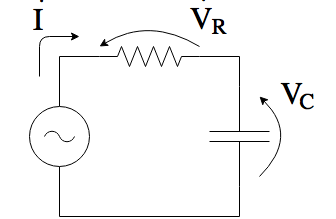
\includegraphics[scale=0.4]{RC_Series_Circuit.png}
  \caption{RC直列回路}
  \label{fig:RC_Series_Circuit2}
\end{figure}
図\ref{fig:fig:RC_Series_Circuit2}に示す回路に、$v = V_m\sin(\omega t + \theta)$の電圧が印加された時、
抵抗、キャパシタンスに加わる電圧の瞬時値を求める式を導出する。

回路の合成インピーダンス $\dot Z$ は
\begin{eqnarray*}
    \dot Z = R + \frac{1}{j\omega C}
\end{eqnarray*}
となり、オームの法則より、電流$\dot I$は
\begin{eqnarray*}
    \dot V = (R + \frac{1}{j\omega C})\dot I\\
    \dot I = \frac{\dot V}{R + \frac{1}{j\omega C}}
\end{eqnarray*}
となる。よって抵抗Rにかかる電圧$\dot V_R$は
\begin{eqnarray*}
  \dot V_R & = & R \dot I\\
  & = & \frac{\dot V}{1 - j\frac{1}{j\omega RC}}
\end{eqnarray*}
となる。ここで、分母を変形する。
\begin{eqnarray*}
  1- j\frac{1}{\omega RC} = \sqrt{1 + (\frac{1}{\omega RC})^2}\angle -(\tan^{-1}(\frac{1}{\omega RC}))
\end{eqnarray*}
よって
\begin{eqnarray*}
  \dot V_R = \frac{\dot V \angle \tan^{-1}(\frac{1}{\omega RC})}{\sqrt{1 + (\frac{1}{\omega RC})^2}}
\end{eqnarray*}
これを瞬時値として表現すると
\begin{eqnarray*}
  v_R = \frac{V_m}{\sqrt{1 + (\frac{1}{\omega RC})^2}} \sin(\omega t + \theta) ただし、\theta = \tan^{-1}(\frac{1}{\omega RC})
\end{eqnarray*}
となる。

同様にキャパシタンスCについて求めると
\begin{eqnarray*}
  v_C = \frac{V_m}{\sqrt{1 + (\omega RC)^2}}\sin(\omega t + \theta) ただし、\theta = \tan^{-1}(\omega RC)
\end{eqnarray*}
となる。

\subsection{式と結果の比較}
先に導出した瞬時値の式と、実験結果(表\ref{tb:result8})を比較する。

$V$については、回路が同等なのでその式は同様に$10.6\sin(6283.185t)$であると考えられる。

$V_R$について、その最大値と$V$との位相差は
\begin{eqnarray*}
  V_R & = & \frac{V_m}{\sqrt{1 + (\frac{1}{\omega RC})^2}}\\
  & \fallingdotseq & \frac{10.6}{1.28}\\
  & \fallingdotseq & 8.28 [V]\\
  \theta_R & = &\tan^{-1}(\frac{1}{\omega RC})\\
  & \fallingdotseq & 0.672 [rad]
\end{eqnarray*}
となる。

同様に$V_C$についても
\begin{eqnarray*}
  V_C & \fallingdotseq & 6.58 [V]\\
  \theta_C & \fallingdotseq & 0.899 [rad]
\end{eqnarray*}
となる。

よってそれぞれの式は、
\begin{eqnarray*}
  v_R(t) = 8.28\sin(6283.185t + 0.672)\\
  v_C(t) = 6.58\sin(6283.185t + 0.899)
\end{eqnarray*}
となる。これを表\ref{tb:result8}の式と比較すると、かなり近い値になっていると考えられる。

\subsection{フェーザ図}
5.2節の実験結果に基づいてフェーザ図を作成した。
以下の図\ref{fig:f}に示す。
\begin{figure}[h]
  \centering
  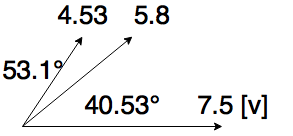
\includegraphics[scale=0.4]{f.png}
  \caption{フェーザ図}
  \label{fig:f}
\end{figure}

\subsection{キャパシタンスと極板面積の関係、測定結果の考察}
キャパシタンスと極板面積の関係は、式
\begin{eqnarray*}
  C = \epsilon_0 \epsilon_r \frac{S}{d}
\end{eqnarray*}
より、比例関係にあるとわかる。

実験に使用した$C_1, C_2$の関係は、
面積が2倍になっているので、そのキャパシタンスの大きさも2倍になると予想できる。
実際の$C_1$のキャパシタンスは、4.86$\times 10^{-13}$、$C_2$のキャパシタンスは2.20$\times 10^{-13}$
であることから、関係は成り立っておらず、コンデンサ作製の際に何らかの不手際があったと考えられる。

\subsection{インダクタンスについて、巻数・コイル長・長岡係数との関係、及び実験との比較}
\begin{eqnarray*}
  L = K \frac{\pi^2 D^2 N^2}{l} \times 10^{-7}
\end{eqnarray*}
式より、インダクタンスは巻数、長岡係数と比例関係にあり、コイル長とは反比例の関係にある。

実験に用いたコイル$L_1, L_2$について、そのインダクタンスを比較すると、$L_2$の巻数が2倍であるので
インダクタンスの値は$L_1$の4倍になると予想できる。

実際のインダクタンスは、$L_1 = 7.77\times 10^{-5}, L_2 = 2.60 \times 10^{-4}$となっており、4倍とまではいかないものの、
巻数によってインダクタンスが大きくなることが確認できた。

\subsection{キャパシタンス$C_1, C_2$直・並列接続時の合成キャパシタンスの式を求め、実験結果と比較する}
直列接続時の合成キャパシタンス$C$は
\begin{eqnarray*}
  C & = &\frac{1}{C_1} + \frac{1}{C_2}\\
  & = &\frac{C_1 C_2}{C_1 + C_2}\\
  & = &\frac{4.86 \times 10^{-13} \times 2.20 \times 10^{-13} }{4.86 \times 10^{-13} + 2.20 \times 10^{-13} }\\
  & = &1.51 \times 10^{-13}
\end{eqnarray*}
\end{document}